\documentclass{proc}
\usepackage{graphicx} % Required for inserting images
\usepackage{array}
\usepackage{hyperref}

\title{IFT3913 - Rapport TP2}
\author{Yalin Mo (20199655) \\ Vennila Sooben (20235256)}
\date{27 octobre 2023}

\begin{document}

\maketitle
\vspace{-7px}
\section{Introduction}
\vspace{-19px}
Dans ce rapport, nous allons détailler notre plan d'évaluation de qualité du projet JFreeChart en utilisant le cadre Objectif-Question-Métrique (GQM). JFreeChart est une bibliothèque de graphiques pour Java créée par Dave Gilbert il y a 23 ans \cite{jfreechart}. Notre objectif est d'analyser la dernière version stable du code de la branche \texttt{master} de JFreeChart pour évaluer sa facilité d'analyse du point de vue du chef du projet. Notez que nous avons utilisé ChatGPT \cite{openai2023} afin d'élaborer un template Latex (titres des sections, préambule...).
\\
Nous commencerons par répondre aux exigences aux exigences de la tâche 1 puis nous enchaînerons avec l'élicitation des réponses obtenues grâce au script. Ensuite, nous analyserons ces résultats pour finir avec une conclusion en nous basant sur les résultats obtenus.

\vspace{-51px}

\section{Plan d'évaluation GQM}
\vspace{-22.5px}
\subsection{Définition des Objectifs}

\begin{tabular}{|c|p{5cm}|}
\hline
\textbf{Champ} & \textbf{Exemple} \\
\hline
Entité analysée & La dernière version stable du code \\
\hline
Objectif de l'analyse & Evaluer \\
\hline
Carac. analysée & Facilité d’analyse  \\
\hline
Point de vue & Chef du projet \\
\hline
Environnement & branche master du JFreeChart \\
\hline
\end{tabular}

\vspace{10px}

Pour la prochaine étape, nous utiliserons les quatre questions spécifiques mentionées dans l'énoncé :

\vspace{-20px}

\subsection{Élicitation des questions}

\subsubsection*{Q1 : Est-ce qu'il y a assez de tests?}
\subsubsection*{Q2 : Les tests sont-ils à jour avec le reste du code?}
\subsubsection*{Q3 : Les tests sont-ils trop complexes?}
\subsubsection*{Q4 : Les tests sont-ils suffisamment documentés?\\}

\subsection{Questions, Métriques et Raisonnement}
Nous avons défini un ensemble de métriques pour chaque question, en nous basant sur les caractéristiques du code de JFreeChart et les exigences de l'évaluation. Voici un aperçu de nos choix de métriques :

\subsubsection*{Q1 : Est-ce qu'il y a assez de tests?}
\begin{itemize}
    \item Réponse 1) \textbf{Ratio test/code}
    \\Raison:
    Nous choisissons cela car nous pouvons connaître intuitivement la proportion de code de test dans tous les fichiers de test. Un ratio élevé peut indiquer une bonne couverture des tests, un ratio faible peut indiquer que le code de test est insuffisant. 
    \item Réponse 2) \textbf{Temps de cycle de test}
    \\Raison:
    Indique le temps nécessaire pour exécuter tous les tests. La longue durée d’exécution des tests peut être due à la grande quantité de code de test. Au contraire, cela peut être dû à un manque de code de test, auquel cas le test peut se terminer dans un délai très court.
    \item Réponse 3) \textbf{Taux de défauts}
    \\Raison:
    Le taux de défauts peut montrer la qualité du fichier de code. Si le taux de défauts après avoir réussi le test est très élevé, c'est-à-dire que certains défauts n'ont pas été détectés par le test, cela peut indiquer que le test n'était pas suffisamment complet.
\end{itemize}

\subsubsection*{Q2 : Les tests sont-ils à jour avec le reste du code?}
\begin{itemize}
   \item Réponse 1) \textbf{Age}
   \\Raison: Ceci va mesurer la période de temps entre la date de création initiale du fichier et la date actuelle. L'âge du code peut être utilisé pour évaluer la stabilité, la maintenance et la pertinence d'une partie spécifique d'un logiciel. Cependant, après avoir éxécuter notre script, nous nous sommes aperçues que les données n'étaient pas utiles (tous identiques).

   \item Réponse 1.2) \textbf{\cite{CodeChurn}Code Churn} (Rotation du Code)
   \\Raison: Etand donné l'échec de 'Age', nous avons choisi Code Churn. Ceci correspond à la fréquence à laquelle des modifications sont apportées à un fichier dans un système de contrôle de version (ici GitHub). Elle mesure le nombre de fois qu'un fichier a été modifié, ajouté ou supprimé au fil du temps. CodeChurn peut aider à évaluer l'activité de développement, l'instabilité d'un fichier, ainsi que les efforts de maintenance et de révision dans un projet logiciel.
   
   \item Réponse 2) \textbf{Temps moyen de test-réparation}
   \\Raison: 
   Cela représente le temps qu'il faut en moyenne pour corriger un test après son échec. Si le temps est long, cela peut signifier que l'écart de temps entre le test et le code modifié est évident, c'est-à-dire que la différence de temps entre leur mise à jour est grande.
   \item Réponse 3) \textbf{Nombre d'échecs de test après modification du code}
   \\Raison:Si ce nombre est élevé, cela peut indiquer que le test ne correspond pas bien au code actuel, ce qui signifie que le test n'est pas mis à jour en temps opportun.
\end{itemize}

\subsubsection*{Q3 : Les tests sont-ils trop complexes?}
\begin{itemize}
   \item Réponse 1) \textbf{Temps d'éxécution des tests}
   \\Raison:
   Le temps d'exécution peut être une bonne explication du problème du code. Si l'exécution des tests prend beaucoup de temps, les tests sont peuvent-être trop complexes ou inefficaces.
   \item Réponse 2) \textbf{Nombre moyen de lignes de cas de test}
   \\Raison:
   Le nombre de lignes de code de test peut refléter intuitivement sa complexité. Trop de lignes par test peuvent indiquer une complexité excessive, rendant le test difficile à comprendre ou à maintenir
\end{itemize}

\subsubsection*{Q4 : Les tests sont-ils suffisamment documentés?}
\begin{itemize}
   \item Réponse 1) \textbf{LOC, CLOC, NLOC}
   \\Raison:
   Ces métriques mesurent différents aspects du code (lignes de code, lignes commentées, lignes non commentées). On peut savoir directement à partir de la réponse si la ligne de commentaire est suffisante. Si la proportion de la ligne de commentaire dépasse les deux autres, cela prouve que les tests sont suffisamment documentés
   \item Réponse 2) \textbf{Couverture du document de test}   
   \\Raison:
   La couverture de la documentation des tests nous aide à comprendre si nos tests couvrent de manière adéquate différentes parties du code. Une couverture élevée de la documentation des tests signifie que nos tests sont détaillés et que chaque partie importante du code a une description de test et de documentation correspondante. Cela garantit que notre code est vérifié dans divers scénarios et que les autres membres peuvent facilement comprendre et exécuter ces tests.
\end{itemize}

Nous avons choisi ces métriques en tenant compte de la pertinence pour chaque question, de leur faisabilité de mesure et de leur coût. Nous passons maintenant à la tâche 2: la mesure deJFreeChart en s'aidant d'un script disponible sur GitHub et dans le dossier de remise (cliquant sur le lien).
\\
\\
Résumé en image:\\
\begin{figure}[htp]
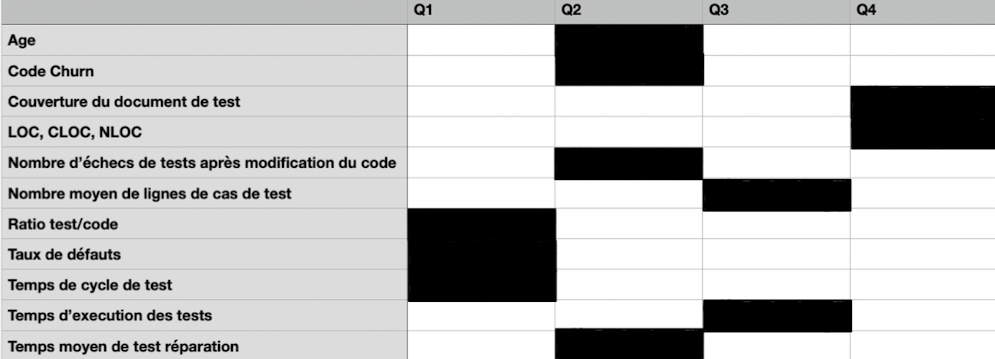
\includegraphics[width=9cm]{metrique.png}
\caption{Tableau Métrique/Question }
\end{figure}
\section{Mesures et Résultats}
Nous avons automatisé le processus de mesure en utilisant divers outils et scripts. Nos résultats de mesure sont les suivants :

\subsection{Résultats pour Q1 : Est-ce qu'il y a assez de tests?}
\begin{itemize}
    \item Réponse 1)\textbf{ Ratio test/code}
    \\Le résultat montre: Le rapport entre le code de test et le code principal est de 0,34. Cela montre que l'investissement du projet dans les tests est faible par rapport au code principal. Un faible ratio peut signifier des tests inadéquats, mais cela peut également varier en fonction de la nature du projet.
    \item Réponse 2)\textbf{ Temps de cycle de test}
    \\Le résultat montre: Le temps d'exécution du test est relativement court d'après les données que nous avons obtenues, et le nombre de fichiers testés est également important, nous pouvons donc résumer grossièrement que le test est suffisant et que la qualité du code est bonne.
    \item Réponse 3)\textbf{ Taux de défauts}
    \\Le résultat montre: Le taux de défauts est 0.00 et le résultat du test mvn montre que tout les tests ont passés.Les deux résultats indiquent  que qualité du code est probablement élevée et il y a assez de tests pour assrer que le programme fonctionne bien.
\end{itemize}

\subsection{Résultats pour Q2 : Les tests sont-ils à jour avec le reste du code?}
\begin{itemize}
    \item Réponse 1) \textbf{Age} : N'a pas aboutie. Toutes les données pour les fichiers étaient quasi les mêmes (jours de commit identique). Pas de conclusion.
    \item Réponse 2) \textbf{Code Churn} : 
Un 'code churn' élevé peut indiquer des activités de développement ou de maintenance continues, tandis qu'un 'code churn' bas peut suggérer un code stable ou dormant. Les données démontrent que certains des tests sont plus complexes car ils ont été modifiés plus de fois notamment CompositeTitleTest.java à 11 (source code one est à 9) contrairement à ImageTitleTest.java à 5(source code à 8) Dans le code, notre max est le fichier TextTitle.java à 14 et min à 7 avec ShortTextTitle.java. Les valeurs étant assez similaires des 2 côtés avec des différences de +-4, nous concluons que \textbf{les tests sont à jour avec le reste du code}.\\
Résumé en image:\\
\begin{figure}[htp]
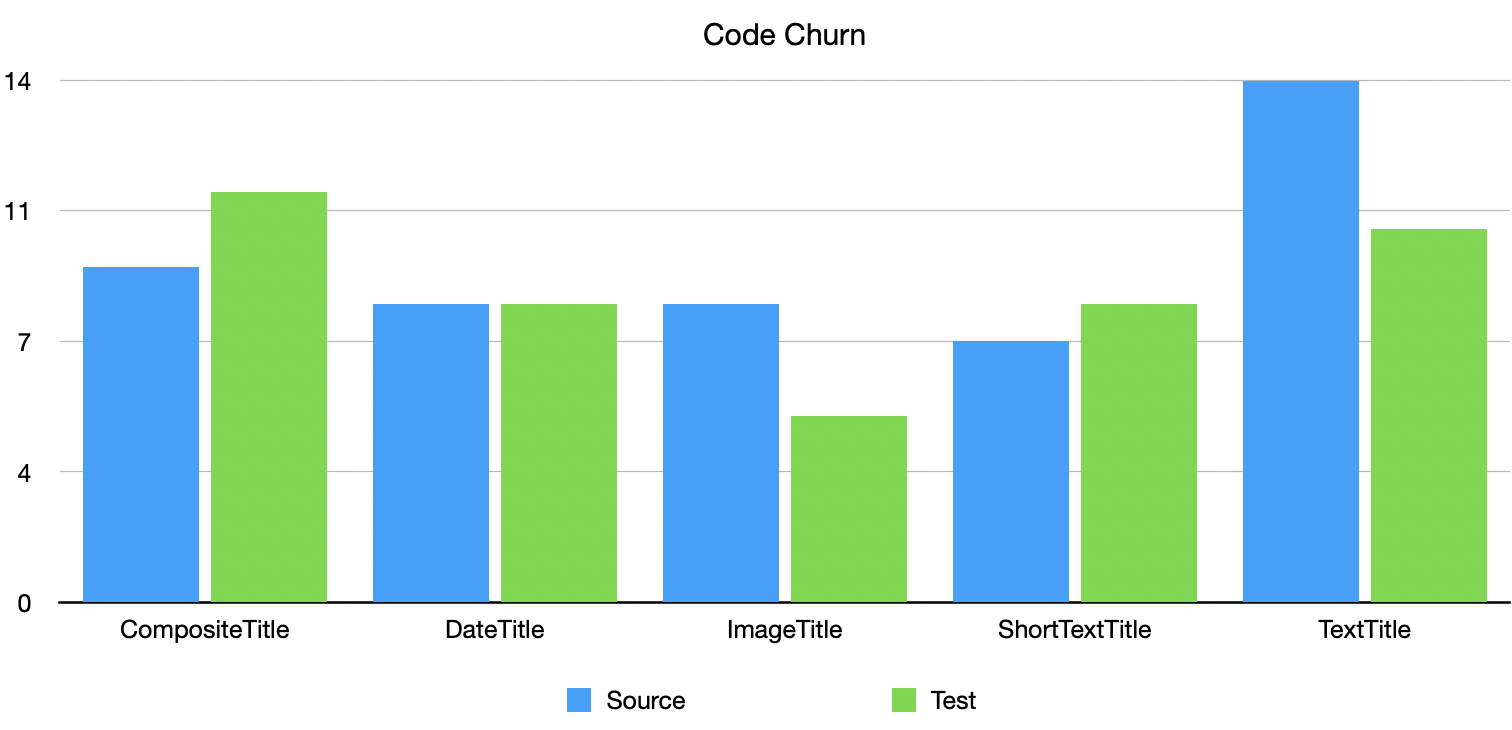
\includegraphics[width=8cm]{codechurn.png}
\caption{Tableau Code Churn Source Code vs Tests }
\end{figure}
    \item Réponse 3) \textbf{Temps moyen de test-réparation}
    \\Le résultat montre: Le temps de correction du code est de 37,27 heures. Selon ce résultat, nous pouvons savoir qu'il n'y a pas beaucoup de décalage horaire entre la création du fichier et la dernière réparation. Nous pouvons résumer grossièrement les tests sont à jour avec le reste du code.
    \item Réponse 4)\textbf{ Nombre d’ échecs de test après modification du code}
    \\Le résultat montre: Les résultats obtenus à l'aide de l'outil SonarQube indiquent que les tests ont réussi même s'il y a des bugs,mais cela a peu d'impact sur le programme. Il ressort des résultats des tests que le nombre d'échecs des tests est très faible, donc nous comcluons que les tests sont à jour avec le reste du code.
\end{itemize}

\subsection{Résultats pour Q3 : Les tests sont-ils trop complexes?}
\begin{itemize}
    \item Réponse 1) \textbf{Temps d'éxécution des tests} : Notre hypothèse de base était : plus de tests = temps d'éxécution plus long. Ceci s'est avéré être vrai (visible dans notre 'scatter diagram' disponible sur le repo github. Les temps restent dans la norme. Une meilleure métrique serait le 'Code Coverage and Execution Time'. Ici nous concluons donc qu'avec notre métrique actuelle, les tests ne sont pas complexes mais reste à determiner.
    \item Réponse 2) \textbf{Nombre moyen de lignes de cas de test}
    \\Le résultat montre: Nombre moyen de lignes de cas de test: 204.76 et l
    e résultat de duplication de l'outil SonarQube montre 8,7\%.
    Le valeur du nombre moyen de lignes de cas de test et la duplication de code sont levés peuvent indiquer une complexité inutile. Le code de test est peut-être complexe. Mais le nombre de fichiers de test affecte également le résultat qu'on a eu. Cela nécessite donc des données supplémentaires pour confirmer si les tests sont complexes.
\end{itemize}

\subsection{Résultats pour Q4 : Les tests sont-ils suffisamment documentés?}
\begin{itemize}
    \item Réponse 1) \textbf{LOC, CLOC, NLOC}: 
    \\ Nous utilisons la commande cloc dans le terminal pour calculer ces trois métriques. Prenons l'exemple du fichier Java, dans les résultats affichés sur le terminal, le nombre de lignes vides dans le fichier est de 26 594, le nombre de lignes de commentaires et de code est de 123 888 et le nombre de lignes de code est de 132 539.
    \\1. LOC (Lignes de code) = code + vide + commentaire = 132539 (ligne de code) + 26594 (ligne vide) + 123888 (ligne de commentaire) = 283021
    \\2. CLOC (Lignes de commentaire de code)= 123888
    \\3. NLOC (Lignes de code sans commentaires) = code + blanc = 132539 (ligne de code) + 26594 (ligne de blanc) = 159133
    \\On peut voir le nombre de lignes commentées du code source, mais cela n'indique pas directement les tests sont bien documentés. Il faut aussi considérer la qualité des commentaires, la complexité du test, etc. Étant donné qu'un test comporte beaucoup de commentaires, il peut ne pas fournir d'informations utiles aux développeurs ou aux testeurs, ou des commentaires détaillés peuvent être fournis dans les tests simples mais pas dans les tests complexes. Nous avons donc besoin d'une analyse plus approfondie à derterminer.
    \item Réponse 2) \textbf{Couverture du document de test}
    \\Le résultat montre:La couverture du document de test: 0.17\%.
    Nous obtenons la couverture du code de test, mais nous ne pouvons pas résumer avec précision si les tests sont suffisamment documentés. Nous supposons que le code de test peut être mieux compris s'il y a plus de fichiers et plus de lignes de code de test. De cet aspect, les tests sont bien documentés.
\end{itemize}

\section{Évaluation de la Facilité d'Analyse}
En combinant les différentes métriques, nous avons évalué la facilité d'analyse de JFreeChart. Notre évaluation est basée sur les réponses aux questions Q1 à Q4. Nous avons utilisé une stratégie d'agrégation qui considère une réponse positive si la majorité des métriques associées à une question indique une performance satisfaisante. Cependant, malgré cette agrégation, certaines zones d'amélioration ont été identifiées.En particulier, bien que le volume de codes de test soit relativement faible pour JFreeChart, les résultats des tests sont positifs car aucun échec n'a été observé. Néanmoins, la couverture de la documentation des tests est faible, signalant un domaine d'amélioration important. Aussi, JFreeChart offre de bonnes performances (pas de crash). De plus, il s'intègre facilement avec d'autres outils tels que Sonerqube. 

\section{Conclusion}
Notre évaluation de la qualité du projet JFreeChart a fourni des informations précieuses sur la facilité d'analyse du code. Certaines parties du code ont montré une bonne qualité de test et de documentation, tandis que d'autres peuvent nécessiter des améliorations. Cette évaluation offre des pistes pour l'amélioration continue du projet. En particulier, une attention accrue pourrait être accordée à la documentation du code et à la réduction du temps de réparation pour faciliter la maintenance et l'adoption du projet par de nouveaux développeurs. S'assurant que tous les tests sont pris en compte par les outils d'analyse de qualité,cela peut réduire efficacement la charge de travail. Cependant, d'un point de vue chef du projet, nous concluons que JFreeChart est facile à analyser bien que pour quelqu'un ayant plus d'expertise technique, elle reste moins simple à analyser.
\\\\
{NB: Nous avons davantage d'images dans le repo git. Le budget de 4 pages ne nous permet pas de les disposer ici}

\bibliographystyle{plain}
\bibliography{references}  

\end{document}
